\chapter{Análisis de los parámetros del algoritmo}

\section{Diversidad}

Recordemos que el objetivo 1 de este trabajo era mejorar la diversidad en problemas de optimización mediante la división de la población en castas.
Mantener la diversidad es crucial para evitar una convergencia prematura hacía un óptimo local. Rosca \cite{Rosca} concluyó que las poblaciones parecían quedar estancadas
en un óptimo local cuando la entropía no cambiaba o decrecía monótonamente en las generaciones sucesivas. En programación genética, la diversidad se refiere a diferencias estructurales, 
como por ejemplo la cantidad de genotipos distintos en la población o la singularidad de valores del fitness \cite{genetic}. Uno de los objetivos de este trabajo es investigar cómo la 
división en castas afecta a la diversidad, así que en esta sección se analizará.  Hay diferentes medidas para calcularla, entre ellas: diversidad genotípica, 
diversidad fenotípica, entropía, pseudo-isomorfismo, distancias de edición, etc. De entre ellas calcularemos la \textbf{entropía}, que describe cómo se distribuye la
población en torno a los diferentes valores del fitness, y la \textbf{distancia de edición}, en la que cada individuo se mide contra el mejor individuo encontrado hasta el 
momento. Se han elegido dado que según Burke \cite{diversity} la entropía y la distancia de edición muestran una gran correlación con el aumento y decremento del valor 
del fitness. Una vez calculadas, se investigará la relación entre el fitness y la diversidad \cite{diversity}. 

\subsection{Experimentos}

Para realizar estas pruebas usaremos la configuración de la Tabla \ref{tab:diversity_config}, como función a minimizar la función Rastrigin \cite{BBOB}, y la distancia euclídea.

\begin{table}[]
    \centering
    \begin{tabular}{||c|c||}
        \hline
        \multicolumn{2}{|l|}{\textbf{Fichero Configuración: config\_file\_5.json} \ref{subsect:config_file_5}} \\ \hline
        Tamaño del cromosoma                            & 20              \\ \hline
        Tamaño de la población                          & 100             \\ \hline
        Máximo de generaciones                          & 15              \\ \hline
        Porcentaje Alfa de la población                 & 10              \\ \hline
        Porcentaje Beta de la población                 & 20              \\ \hline
        Porcentaje Gamma de la población                & 20              \\ \hline
        Porcentaje Delta de la población                & 20              \\ \hline
        Porcentaje Epsilon de la población              & 30              \\ \hline
        Tasa de mutación                               & 10              \\ \hline
    \end{tabular}
    \caption{Parámetros de configuración para exploración de la diversidad}
    \label{tab:diversity_config}
\end{table}

\begin{figure}[H]
	\centering	
	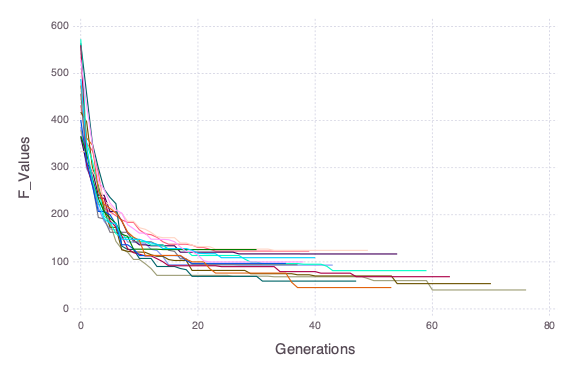
\includegraphics[scale=0.6]{../data/Plots/config_file_5_Rastrigin.png}
	\caption{Primera ejecución}
    \label{fig:primera_ejecucion}
\end{figure}

En la Figura \ref{fig:primera_ejecucion} se ve el resultado de ejecutar el algoritmo 15 veces con la configuración anterior.
Se puede observar cómo los mejores resultados se obtienen en las primeras generaciones. La mayoría de las ejecuciones muestran cómo la mejora
del fitness disminuye alrededor de la generación 15-20. Esto puede indicar que cuanto mayor es la generación menor es la diversidad. 
Para apoyar esta idea tenemos las Figuras \ref{fig:best_f_value} y \ref{fig:worst_f_value}. 

La Figura \ref{fig:best_f_value} muestra la diversidad de la ejecución que resulta en un mejor fitness. De la generación 0 a la 30 se produce un decremento de la entropía,
pero se vuelve a recuperar en el resto de generaciones. La entropía empezando y acabando casi con el mismo valor nos dice que el algoritmo mantiene una diversidad similar a 
lo largo de toda la ejecución, lo que puede dar lugar a mejores resultados. En la Figura \ref{fig:worst_f_value}, que muestra la peor ejecución, podemos 
ver un comportamiento similar; el descenso también se produce en las generaciones 0-25. 

\begin{table}[]
    \begin{tabular}{||c|c|c|c|c|c||}
    \hline
                                                                            & \textbf{\begin{tabular}[c]{@{}c@{}}Evals. de \\ f\end{tabular}} & \textbf{Entropía} & \textbf{\begin{tabular}[c]{@{}c@{}}Distancia de \\ edición\end{tabular}} & \textbf{Mejor f} & \textbf{Generaciones} \\ \hline
    \textbf{\begin{tabular}[c]{@{}c@{}}Mejor \\ ejecución\end{tabular}}     & 11873                & 2.69              & 6.20                          & 40.27                     & 77                    \\ \hline
    \textbf{\begin{tabular}[c]{@{}c@{}}Peor \\ ejecución\end{tabular}}      & 4900                 & 2.11              & 5.95                          & 126.14                    & 31                    \\ \hline
    \end{tabular}
    \caption{Comparación de la ejecución con mejor valor de fitness y la peor, usando el fichero de configuración 5 [\ref{subsect:config_file_5}]}
    \label{fig:Comparación}
\end{table}

En ambas imágenes la distancia de edición mantiene una correlación estrecha con el valor del fitness, y en ambos casos acaba con unos valores similares. Mirando la tabla \ref{fig:Comparación}, y las figuras
mencionadas no se puede concluir una diferencia clave que marque el por qué una es la mejor ejecución y otra la peor.

\begin{figure}[]
	\centering	
	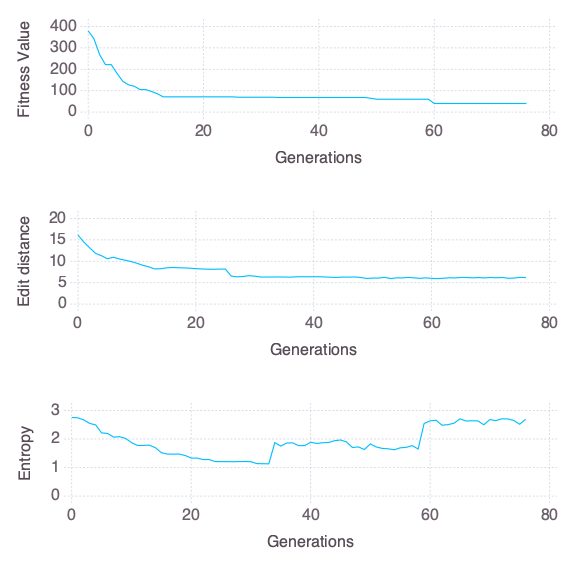
\includegraphics[scale=0.5]{../data/Plots/config_file_5_Rastrigin_best_f_value.png}
	\caption{ Diversidad en la ejecución con mejor resultado de fitness }
    \label{fig:best_f_value}
\end{figure}

\begin{figure}[]
	\centering	
	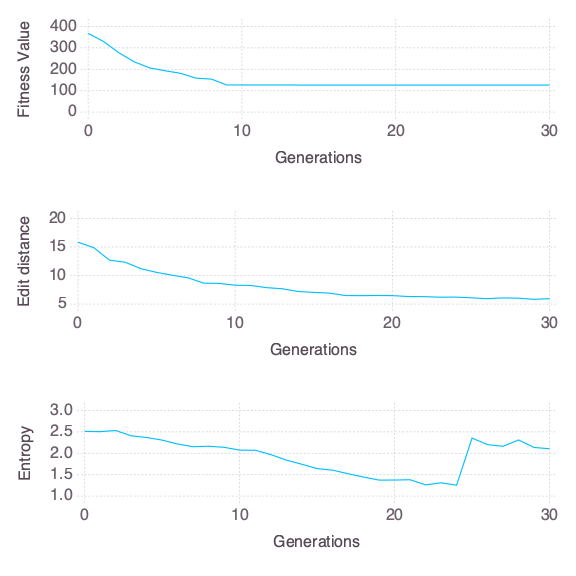
\includegraphics[scale=0.5]{../data/Plots/config_file_5_Rastrigin_worst_f_value.png}
	\caption{ Diversidad en la ejecución con peor resultado de fitness }
    \label{fig:worst_f_value}
\end{figure}

\section{Exploración Inicial}

El objetivo de esta exploración es escoger los parámetros: dimensión del cromosoma (\textit{DIM}) y tamaño de población. Primero se varía la dimensión
del cromosoma y la población se mantiene fija a 100. Se ejecutará el algoritmo 15 veces por cada dimensión del cromosoma, y se cogerá el que 
tenga mejor resultado para la comparación. Los resultados de esta primera exploración se encuentran en la Tabla \ref{tab:fitness_variation}. 

\begin{table}[]
    \centering
    \begin{tabular}{||c|c|c|c|c|c||}
        \hline
        \textbf{Fichero Configuración} & \textbf{Generaciones} & \textbf{DIM} & \textbf{Mejor fitness} & \textbf{Evals. de f}\\ \hline
        Config 1   & 16    & 2   & -76.93    &  2340  \\ \hline
        Config 2   & 20    & 3   & -74.70    &  2900  \\ \hline
        Config 3   & 20    & 5   & -67.58    &  2900  \\ \hline
        Config 4   & 56    & 10  & -45.74    &  8567  \\ \hline
        Config 5   & 68    & 20  & 49.43     &  10494 \\ \hline
        Config 6   & 52    & 40  & 422.26    &  8133  \\ \hline
    \end{tabular}
    \caption{Resultados exploración inicial}
    \label{tab:fitness_variation}
\end{table}

\begin{figure}[]
	\centering	
	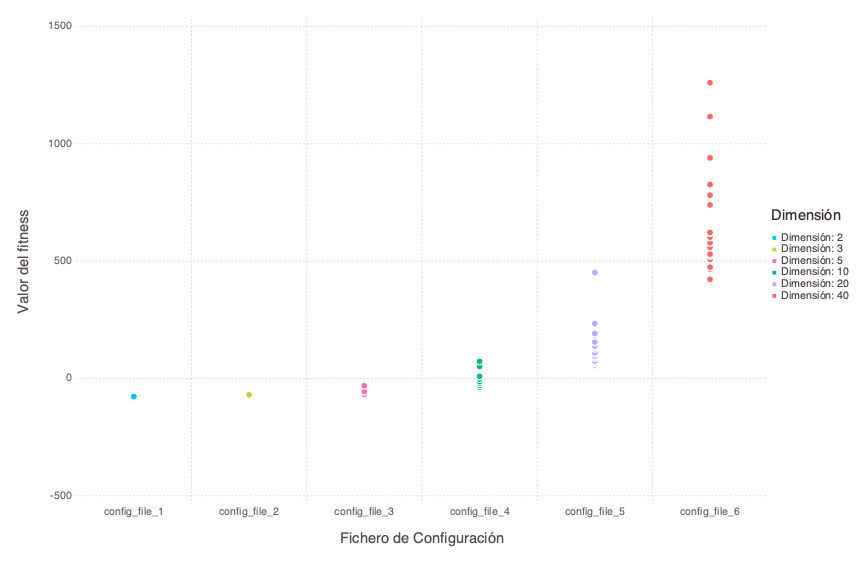
\includegraphics[scale=0.4]{figuras/config_file_1-6_Rastrigin_box_plots.png}
	\caption{ Variación del valor del fitness }
    \label{fig:box_plots}
\end{figure}

Para un tamaño de población 100 aparentemente la mejor dimensión es la 3. Sin embargo, mirando la Figura \ref{fig:box_plots} vemos
que la configuración 2 apenas ha explorado el espacio, ha alcanzado un óptimo local, al igual que de la 1 a la 3. Para
futuras explotaciones descartaremos estas configuraciones, ya que no aportan apenas información sobre el comportamiento del algoritmo.
Con la información extraída de estos experimentos no se puede concluir qué valores escoger para el tamaño de población ni para la
dimensión del cromosoma escoger. En las siguientes secciones se le dará un enfoque diferente.
\section{Exploración del tamaño de población}

\begin{table}[]
    \centering
    \begin{tabular}{|c|c|c|c|c|c|}
        \hline
        \textbf{Config.} & \textbf{\begin{tabular}[c]{@{}c@{}}Tmñ.\\ Población\end{tabular}} & \textbf{\begin{tabular}[c]{@{}c@{}}Mediana \\ mejor valor \\ de fitness\end{tabular}} & \textbf{\begin{tabular}[c]{@{}c@{}}Mediana \\ \# ejecuciones \\ de f\end{tabular}} & \textbf{\begin{tabular}[c]{@{}c@{}}$\sigma$\\ mejor valor\\ de fitness\end{tabular}} & \textbf{\begin{tabular}[c]{@{}c@{}}$\sigma$\\ \# ejecuciones \\ de f\end{tabular}} \\ \hline
        4  [\ref{subsect:config_file_4}]                & 100                                                               & 7.00                                                                                  & 7852.0                                                                             & 11.98                                                                         & 2045.87                                                                     \\ \hline
        7  [\ref{subsect:config_file_7}]                & 150                                                               & 0.27                                                                                  & 9010.0                                                                             & 15.10                                                                         & 2536.42                                                                     \\ \hline
        8  [\ref{subsect:config_file_8}]                & 300                                                               & -18.06                                                                                & 23496.0                                                                            & 10.20                                                                         & 6406.70                                                                     \\ \hline
        9  [\ref{subsect:config_file_9}]                & 500                                                               & -26.11                                                                                & 37087.0                                                                            & 5.61                                                                          & 8492.77                                                                     \\ \hline
        10 [\ref{subsect:config_file_10}]               & 1000                                                              & -33.53                                                                                & 75539.5                                                                            & 5.63                                                                          & 21178.32                                                                    \\ \hline
    \end{tabular}
    \caption{Resultados exploración inicial para diferentes tamaños de población}
    \label{tab:base_population}
\end{table}

El objetivo de esta sección es obtener una población inicial base para las próximas exploraciones. Dejaremos fija la dimensión del cromosoma a 10 y
ejecutaremos cada fichero de configuración 15 veces. Se ha escogido esta dimensión porque ha alcanzado una solución 
relativamente buena en el experimento anterior. Las soluciones de esta exploración se encuentran en la Tabla \ref{tab:base_population}. 
En esta nueva exploración se han probado los tamaños de población: 100, 150, 300, 500, 1000, indicados en la Tabla \ref{tab:base_population}
como \textit{Tmñ. poblacion}. En la Figura \ref{fig:population_size_variation} se vuelve a ver cómo el mayor descenso del valor del fitness se produce
entre la generación 0 y la 20. La población con tamaño 1000 (Config 10 en Tabla \ref{tab:base_population}) es la que tiene
un mayor descenso pasada la generación 20. 

\begin{figure}[]
	\centering	
	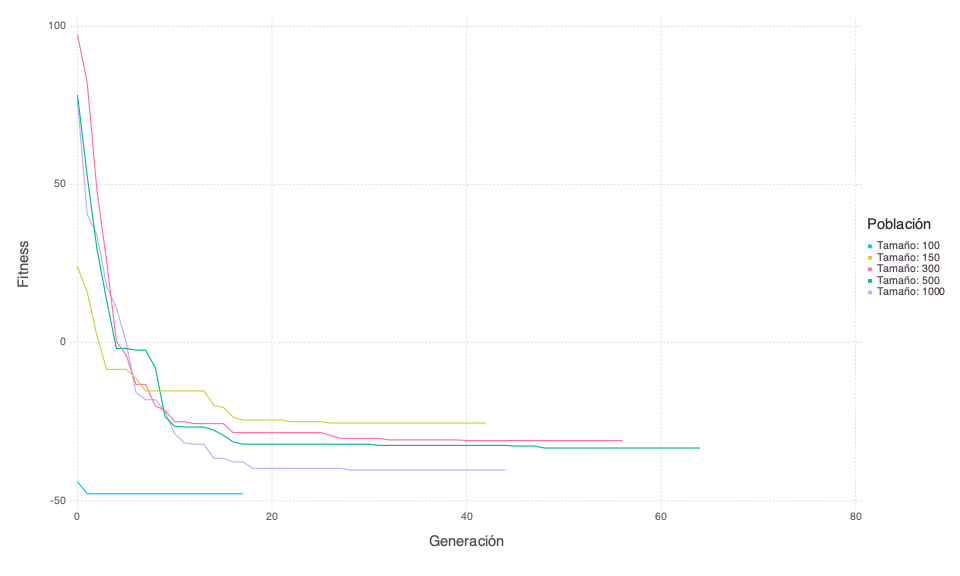
\includegraphics[scale=0.5]{../data/Plots/population_size_variation.png}
	\caption{ Ejecuciones variando el tamaño de la población }
    \label{fig:population_size_variation}
\end{figure}

En la Figura \ref{fig:population_size_box_plots}, se ve que la configuración 4 [\ref{subsect:config_file_4}] es la que alcanza un valor más pequeño de fitness.
Sin embargo mirando la Tabla \ref{tab:base_population} es la configuración 10 [\ref{subsect:config_file_10}] la que tiene mejor mediana para el valor del 
fitness, y además menor desviación típica, por lo que en general se mueve por solciones relativamente buenas.

\begin{figure}[]
	\centering	
	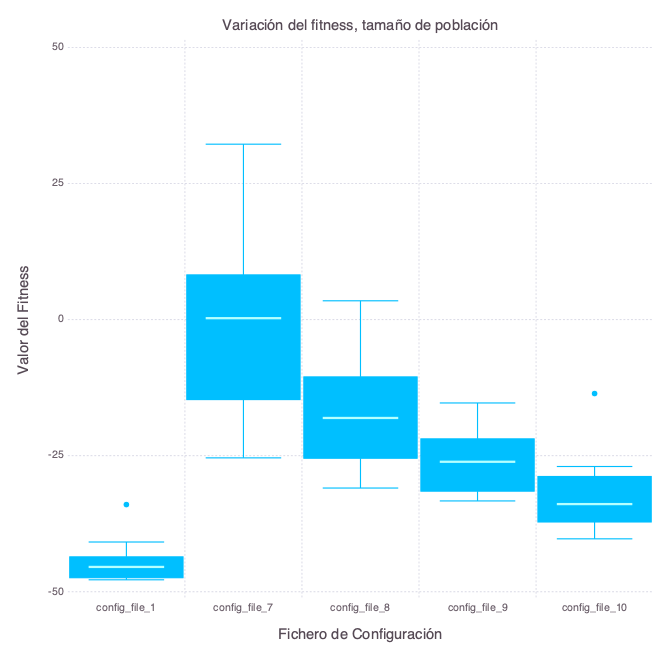
\includegraphics[scale=0.5]{../data/Plots/Rastrigin_box_plots_p_size.png}
	\caption{ Diversidad en la ejecución variando el tamaño de población }
    \label{fig:population_size_box_plots}
\end{figure}


El objetivo de esta exploración era sacar una población inicial en la que basar el resto de experimentos. Por tanto atendiendo al que tiene mejor mediana,
usaremos la configuración 10 [\ref{subsect:config_file_10}] para las siguientes exploraciones.
\input{secciones/exploracion_tamaño_cromosoma.tex}
\section{Exploración de la tasa de mutación}

\section{Análisis de las soluciones}

- Variar la mutacion.
- En que casos da mejor resultado y por qué, comparar con hipótesis inicial.
- Por qué da mejores resultados con una función o con otra o con respecto al algoritmo genético.
